\chapter{Resultados}

    En el capítulo anterior se detalló el proceso de construcción de dos modelos de red a partir de los datos GTFS: el L-espacio, que representa la infraestructura física, y el P-espacio, que modela la conectividad del servicio.

    Este capítulo presenta los resultados de aplicar un conjunto de análisis estructurales a ambos grafos. El objetivo es caracterizar y comparar las propiedades de cada modelo para obtener una comprensión más profunda de la red de transporte. Se abordan cuatro áreas principales: el cálculo de métricas globales, el análisis de centralidad, la detección de comunidades y la evaluación de la robustez de la red.


    \section{Análisis del L-espacio: La Red de Infraestructura}
        En esta sección se presentan los resultados del análisis aplicado al grafo L-espacio, que modela la contigüidad física de la red de paradas y rutas.

        \subsection{Métricas globales del L-espacio}
        El primer objeto de nuestro análisis es el conjunto de paradas y estaciones del sistema de transporte público. En concreto, nos interesa saber qué tan bien conectadas están con el resto de la infraestructura, qué tan accesibles son en términos de distancia y cómo se distribuye la infraestructura en el espacio.

        \subsubsection{Conectividad y Estructura General}
            Las métricas iniciales revelan una visión panorámica de la red:
            \begin{itemize}
                \item \textbf{Tamaño de la Red:} El grafo consolidado consta de \textbf{4,203 nodos} (supernodos que agrupan paradas) y \textbf{8,591 aristas} (conexiones directas por una ruta).
		\item \textbf{Densidad del Grafo:} La densidad es de \textbf{0.000486}, un valor esperado. Esto es así porque en el grafo que estamos estudiando, dos nodos solamente están conectados si sus estaciones correspondientes están conectadas por una ruta que vaya directamente de uno a otro. Es decir, cada nodo tiene por lo general dos conexiones. Es posible que un supernodo tenga más conexiones, pues aglomera varias paradas, pero el número de estas conexiones está acotado por el número de paradas que aglomera; en el peor de los casos, un supernodo tiene dos conexiones por cada ruta que lo atraviesa.
                \item \textbf{Conectividad:} El análisis de componentes conectados arrojó un resultado clave: la red está fragmentada en \textbf{2 componentes}. Uno de ellos es masivo, conteniendo 4,198 nodos (el 99.8\% del total), mientras que el segundo es un fragmento aislado de apenas 5 nodos. Esto sugiere que, en la práctica, la red funciona casi como un todo unificado, pero existe una pequeña \textit{isla} de paradas sin conexión con el resto del sistema.
                \item \textbf{Coeficiente de Clustering Global:} La transitividad de la red es de \textbf{0.1088}. Este valor, cercano a cero, indica una baja tendencia a la formación de clústeres locales. En otras palabras, es poco probable que dos paradas conectadas a una tercera estén también conectadas entre sí. Esto sugiere una topología de red más arbórea o con forma de estrella (\textit{hub-and-spoke}) que una estructura de malla densa, lo cual puede indicar que la red se centra en conectar zonas periféricas con otras más centrales. 
            \end{itemize}

        \subsubsection{Eficiencia y Tiempos de Viaje}
            Además de las propiedades vistas antes, nos interesa saber qué tan alejadas están entre sí cualesquiera dos paradas o estaciones. Esto puede responderse fijándose en varias métricas que vemos a continuación:
            \begin{itemize}
                \item \textbf{Conectividad Fuerte:} Un detalle importante es que el grafo principal no es \textit{fuertemente conectado}. Esto significa que existen pares de nodos (A, B) para los cuales es posible viajar de A a B, pero no hay una ruta de regreso de B a A. Este fenómeno es común en sistemas de autobuses debido a la existencia de calles de un solo sentido o circuitos de ruta.
                \item \textbf{Diámetro de la Red:} El diámetro, medido en el componente principal, es de \textbf{77 saltos}. Representa el número máximo de supernodos que se deben atravesar en el peor de los casos para conectar dos puntos de la red. Algo que nos indica esta cifra es que el sistema de transporte público abarca una zona extensa de territorio, lo que por otro lado sabemos porque conocemos la extensión de la Zona Metropolitana de Guadalajara.
                \item \textbf{Índice de Desvío Promedio (Detour Index):} Se obtuvo un valor de \textbf{1.13}. Un valor de 1 representa un viaje en línea recta; este índice indica que, en promedio, los viajes son 13\% más largos que la distancia directa, lo que refleja rutas relativamente directas pero con margen para mejorar conexiones.
            \end{itemize}

        \subsubsection{Accesibilidad y Cobertura de la Red (Matriz de Shimbel)}
            El análisis de la matriz de distancias de Shimbel, que contiene los tiempos de viaje más cortos entre todos los pares de nodos, permite evaluar la accesibilidad desde la perspectiva del usuario en términos de tiempo de viaje:
            \begin{itemize}
                \item \textbf{Nodos más y menos accesibles:} Se identificó una brecha extrema en la accesibilidad. Los \textbf{nodos mejor conectados} promedian entre \textbf{0.7 y 1.3 minutos} al resto de la red. En contraste, los \textbf{nodos peor conectados}, situados en la periferia (Tesistán, aeropuerto, norponiente), promedian entre \textbf{94 y 157 minutos}.
                \item \textbf{Análisis de Cobertura:} Se calculó el porcentaje de la red accesible desde una parada promedio en distintos umbrales de tiempo:
                \begin{itemize}
                    \item \textbf{15 minutos:} Se alcanza solo el 6.5\% de la red.
                    \item \textbf{30 minutos:} Se alcanza el 33.1\% de la red.
                    \item \textbf{45 minutos:} Se alcanza el 61.9\% de la red.
                    \item \textbf{60 minutos:} Se alcanza el 80.1\% de la red.
                \end{itemize}
                Estos datos muestran que el umbral de 45-60 minutos es crítico para acceder a la mayor parte de la ciudad, mientras que el acceso a oportunidades en viajes cortos (menos de 30 minutos) es considerablemente limitado.
                \item \textbf{El Viaje más Largo:} El trayecto más largo posible dentro de la red toma \textbf{244 minutos (más de 4 horas)}, conectando una zona relativamente céntrica con la periferia norponiente. Este caso extremo subraya la enorme escala de tiempo que implica atravesar la ciudad y la ineficiencia de ciertas conexiones específicas.
            \end{itemize}

	    En resumen, los indicadores muestran que el sistema de transporte público es extenso y está bien distribuido en el espacio, aunque también es desigual. La alta arboricidad de la red sugiere que las rutas están pensadas principalmente para conectar las zonas céntricas de los distintos municipios con sus respectivas periferias. Una consecuencia de esto es que muchos caminos deben pasar por esas zonas céntricas para acceder al resto de la red, lo que alerta sobre posibles cuellos de botella, aglomeraciones y sobredemanda.

            Este diagnóstico conecta directamente con el concepto de \textit{centralidad} introducido en el capítulo 1. De ese concepto se echará mano a continuación para evaluar si estos cuellos de botella existen y, de existir, dónde se concentran.

        \subsection{Análisis de Centralidad en el L-espacio}
            A diferencia de las métricas globales, el análisis de centralidad se enfoca en la importancia relativa de cada nodo dentro de la red. Un nodo puede ser "importante" por distintas razones: por ser un punto de alto tráfico, por actuar como un puente crítico, por su cercanía al resto del sistema o por su influencia en corredores clave. A continuación, se analizan cuatro tipos de centralidad, cada una revelando una faceta distinta de la estructura de la red. Los resultados fueron calculados para cada uno de los 4,203 nodos.

        \subsubsection{Centralidad de Grado Ponderado}
            Esta es la medida más directa de la actividad de un nodo. En lugar de solo contar las conexiones, se pondera cada una por el atributo \texttt{original\_edge\_count}, que representa el número de rutas reales que conforman esa arista consolidada. Así, el grado ponderado refleja el \textbf{volumen total de rutas} que atiende una parada.
            \begin{itemize}
                \item \textbf{Hallazgos Clave:} Los nodos con mayor grado ponderado no solamente se encuentran en el centro de la ciudad, sino en las \textbf{intersecciones viales más importantes}. Puntos como la Nueva Central Camionera, Estación Periférico Sur, o la zona de López Mateos y Las Águilas, emergen como los principales distribuidores de tráfico, donde converge físicamente el mayor número de líneas de autobús.
            \end{itemize}

        \subsubsection{Centralidad de Intermediación}
            Esta métrica identifica los nodos que con mayor frecuencia se encuentran en los caminos más cortos (en tiempo de viaje) entre otros pares de nodos. Son los \textbf{puentes y puntos de transbordo más críticos} de la red. Para su cálculo, se utilizó el tiempo de viaje (\texttt{travel\_time\_minutes}) como peso, identificando así los nodos cruciales para las rutas más rápidas.
            \begin{itemize}
                \item \textbf{Hallazgos Clave:} El \textbf{Centro Histórico} emerge como el corazón neurálgico para los transbordos. Nodos situados en Av. 16 de Septiembre y sus alrededores obtuvieron las puntuaciones más altas. Aunque no manejan el mayor volumen de rutas (grado), son los puntos por los que es necesario pasar para conectar eficientemente distintas zonas de la ciudad, funcionando como las articulaciones principales del sistema.
            \end{itemize}

            La pregunta en este punto es: ¿qué supernodos concentran simultáneamente volumen de rutas e intermediación para sostener los transbordos del sistema? La Figura~\ref{fig:centralidad_b_l_space} responde esa pregunta al escalar por grado ponderado y colorear por centralidad de intermediación; esta lectura habilita priorizar supernodos para protección operativa y mantenimiento preventivo.
            \begin{figure}[h!]
                \centering
                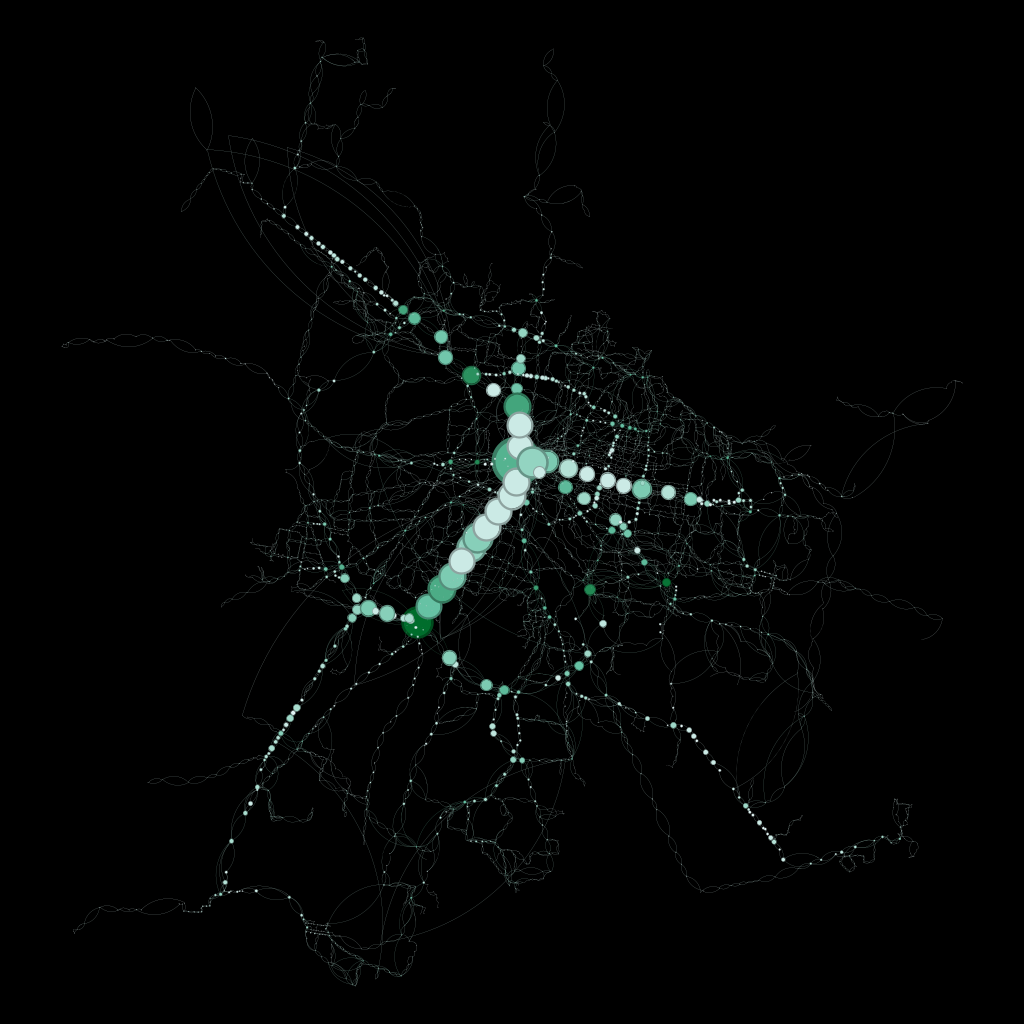
\includegraphics[width=\textwidth]{../../grafos/l_space/grafo_centralidades_betweness.png}
                \caption{L-espacio: tamaño del supernodo proporcional al grado ponderado y color verde proporcional a la centralidad de intermediación. La lectura conjunta permite ubicar supernodos puente cuya falla puede incrementar transbordos y debilitar la conectividad entre corredores.}
                \label{fig:centralidad_b_l_space}
            \end{figure}

        \subsubsection{Centralidad de Cercanía (Closeness Centrality)}
            Mide qué tan cerca está un nodo, en promedio, de todos los demás nodos alcanzables, usando el tiempo de viaje como distancia. Un nodo con alta centralidad de cercanía es aquel desde el cual se puede llegar \textbf{más rápidamente} al resto de la red.
            \begin{itemize}
                \item \textbf{Hallazgos Clave:} Los resultados son contundentes: los nodos con la mayor centralidad de cercanía se concentran de manera casi exclusiva en el \textbf{hipercentro de la ciudad}. Esto confirma que, en términos de tiempo de viaje, el centro es el punto más accesible y el verdadero "kilómetro cero" de la red de transporte público, desde donde el tiempo promedio para alcanzar cualquier otro destino es el más bajo. Algo a destacar es que la diferencia entre los distintos nodos con respecto a esta centralidad no es tan radical como en otras medidas.
            \end{itemize}

        \subsubsection{Centralidad de Eigenvector (Eigenvector Centrality)}
            Esta métrica asigna importancia a un nodo en función de la importancia de sus vecinos. Un nodo es importante si está conectado a otros nodos importantes. Para su cálculo se ponderó por el número de rutas agregadas en cada arista consolidada. Con ello se privilegian las conexiones multirruta.
            \begin{itemize}
                \item \textbf{Hallazgos Clave:} De manera sorprendente, esta métrica no destacó al centro ni a los grandes cruceros. En su lugar, reveló la existencia de un \textbf{corredor de alta influencia en Av. Mariano Otero}, al sur de Las Águilas. Los nodos en esta zona obtuvieron las puntuaciones más altas, indicando que no solo son importantes individualmente, sino que juntos forman la "columna vertebral" de un subsistema de nodos muy influyentes, conectando de manera robusta el sur y poniente de la ciudad.
            \end{itemize}

            La pregunta comparativa aquí es: ¿en qué corredores coinciden accesibilidad temporal e influencia estructural? La Figura~\ref{fig:centralidad_c_l_space} responde al colorear supernodos por cercanía y escalarlos por eigenvector; esta lectura habilita decidir dónde concentrar acciones para reducir tiempos de viaje sin debilitar enlaces críticos.
            \begin{figure}[h!]
                \centering
                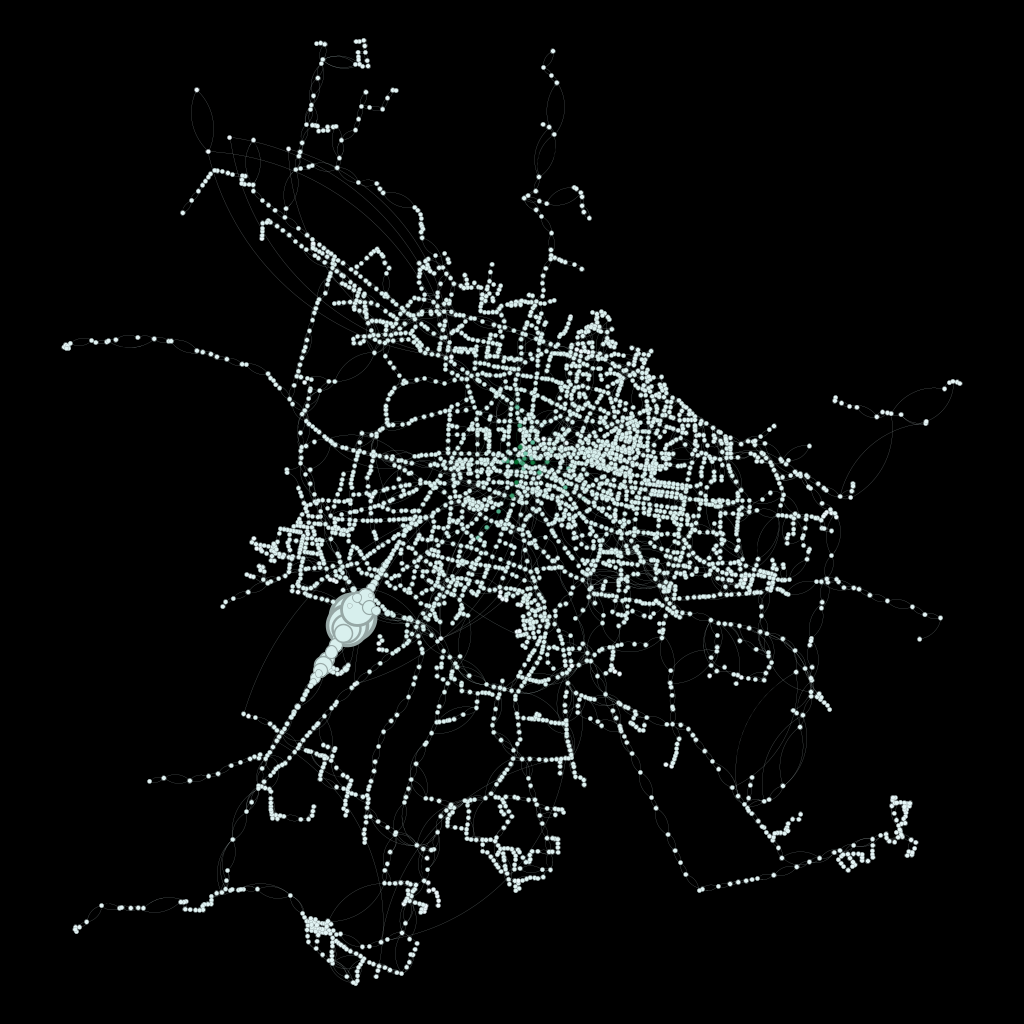
\includegraphics[width=\textwidth]{../../grafos/l_space/grafo_centralidades_closeness.png}
                \caption{L-espacio: color verde según centralidad de cercanía y tamaño del supernodo según centralidad de eigenvector. La figura permite distinguir corredores desde los que conviene mejorar accesibilidad temporal y, al mismo tiempo, preservar influencia estructural.}
                \label{fig:centralidad_c_l_space}
            \end{figure}

            En síntesis, el análisis de centralidades descompone la "importancia" en roles especializados: el Centro Histórico es el núcleo de la \textbf{accesibilidad y los transbordos} (Cercanía e Intermediación), las grandes avenidas son los centros de \textbf{volumen} (Grado), y corredores específicos como Mariano Otero funcionan como los \textbf{ejes de influencia} estructural (Eigenvector).

        \subsection{Detección de Comunidades en el L-espacio}
            El siguiente paso en el análisis es determinar si la red se agrupa en sub-redes o clústeres. Una comunidad en un grafo es un conjunto de nodos que están más densamente conectados entre sí que con el resto de la red. En el contexto del transporte público, estas comunidades suelen corresponder a zonas geográficas coherentes, corredores de alta frecuencia o subsistemas de rutas.

            Para identificar estas estructuras, se utilizó el \textbf{método de Louvain}, un algoritmo ampliamente reconocido por su eficiencia y precisión en la detección de comunidades en grafos a gran escala. El algoritmo optimiza la \textit{modularidad} de la red, una métrica que cuantifica la calidad de una partición en comunidades. Se aplicó sobre una versión no dirigida del grafo, utilizando el atributo \texttt{original\_edge\_count} como peso para que las comunidades se formaran en torno a los flujos de rutas más significativos.

        \subsubsection{Resultados de la Detección}
            El análisis arrojó los siguientes resultados clave:
            \begin{itemize}
                \item \textbf{Número de Comunidades:} Se detectaron un total de \textbf{40 comunidades}. La gran mayoría de ellas (39) son significativas en tamaño, mientras que solo una fue identificada como un pequeño grupo aislado de menos de 5 nodos, probablemente correspondiente al componente desconectado mencionado en la sección de métricas globales.
                \item \textbf{Estructura Policéntrica:} La existencia de un número considerable de comunidades robustas confirma que la red no es monolítica, sino que posee una \textbf{estructura policéntrica}. En lugar de un único núcleo dominante, el sistema se organiza en torno a múltiples centros o zonas funcionales.
                \item \textbf{Comunidades Principales:} Las 10 comunidades más grandes agrupan a más de 1,800 nodos, casi la mitad de la red. El análisis de sus centroides geográficos permite una caracterización preliminar:
                \begin{itemize}
                    \item La comunidad más grande (245 nodos) tiene su centro en la zona de \textbf{San Juan de Dios y el Hospicio Cabañas} (Lat: 20.68, Lon: -103.31), abarcando el oriente del centro histórico.
                    \item Otras comunidades importantes se localizan en el \textbf{corredor de Plaza del Sol y la Expo} (Com. 35), el \textbf{centro de Guadalajara} (Com. 9), la zona de \textbf{San Andrés y el oriente de la ciudad} (Com. 8), el sur de \textbf{Zapopan} (Com. 20 y 37), y los centros de \textbf{Tlaquepaque} (Com. 10 y 11) y \textbf{Tonalá}.
                    \item Una comunidad notable (Com. 33) se extiende hacia el norte, en la zona de \textbf{Tesistán}, representando un subsistema periférico bien definido.
                \end{itemize}
            \end{itemize}

            En conclusión, la detección de comunidades revela la organización interna de la red de transporte. Muestra cómo el sistema se articula en subsistemas geográficos que corresponden en gran medida a la división municipal y a los grandes corredores viales del Área Metropolitana de Guadalajara. Esta granularidad es fundamental para entender los patrones de viaje a una escala intermedia, más allá del nivel de parada individual pero más específico que el de la red completa.

            La pregunta territorial es: ¿qué bloques de supernodos están más cohesionados por rutas compartidas y dónde conviene focalizar seguimiento? La Figura~\ref{fig:comunidades_l_space} lo muestra con comunidades por modularidad y grosor de arista según rutas compartidas, habilitando decisiones de monitoreo e intervención por subsistemas.

            \begin{figure}[h!]
                \centering
                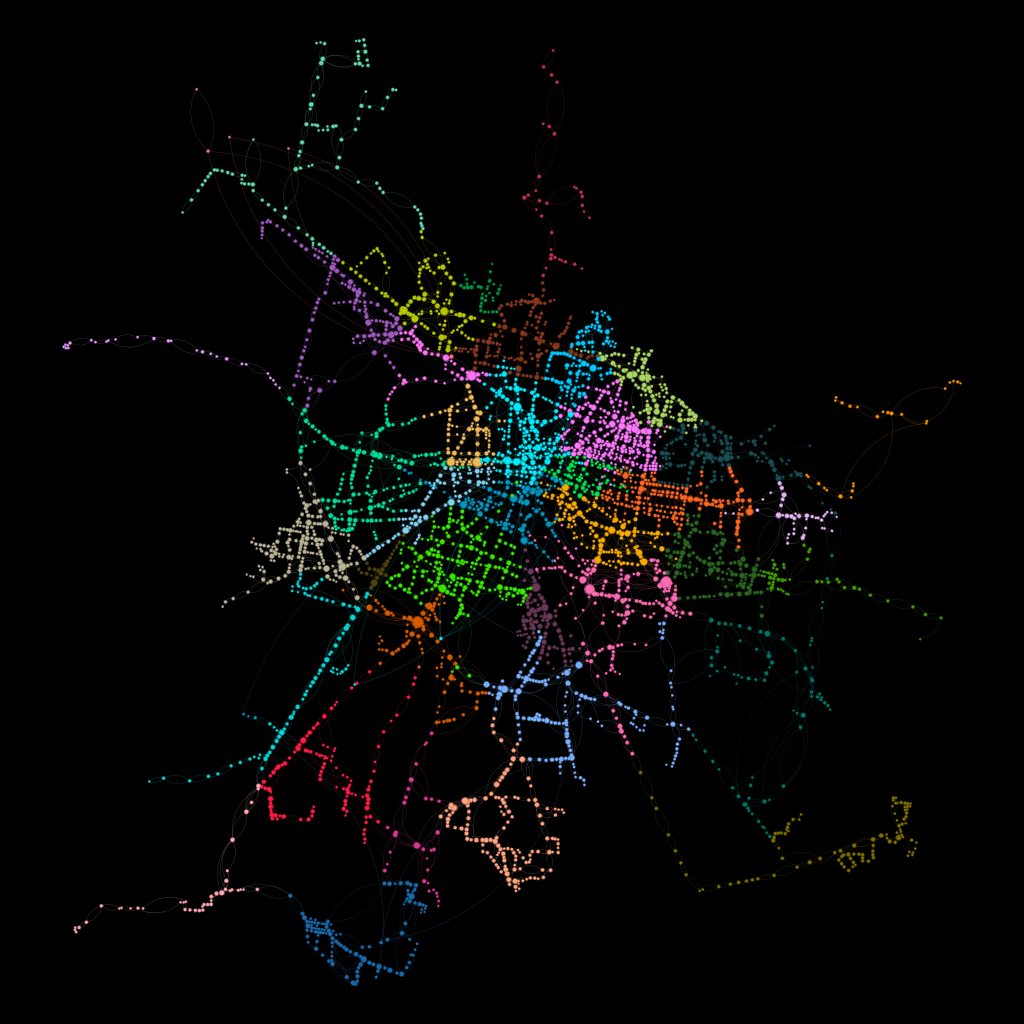
\includegraphics[width=\textwidth]{../../grafos/l_space/grafo.png}
                \caption{Comunidades del L-espacio detectadas con Louvain: color por comunidad y grosor de arista según número de rutas compartidas. La visualización facilita delimitar subsistemas territoriales para seguimiento diferenciado de conectividad y operación.}
                \label{fig:comunidades_l_space}
            \end{figure}

        \subsection{Análisis de Robustez del L-espacio}
            Una vez caracterizada la estructura estática de la red, el siguiente paso es evaluar su resiliencia. Un sistema de transporte robusto es aquel que puede mantener su funcionalidad principal —conectar personas y lugares de manera eficiente— incluso cuando algunas de sus partes fallan. Para medir esta robustez, se simularon ataques dirigidos que eliminan nodos críticos y se observó el impacto en la conectividad y eficiencia de la red.

        \subsubsection{Metodología de la Simulación}
            Se eliminan de manera secuencial los \textbf{50 nodos con mayor grado ponderado}, que son los supernodos con más rutas incidentes. Tras cada eliminación se recalcula:
            \begin{itemize}
                \item \textbf{Tamaño del Componente Conectado Gigante (LCC):} proporción del LCC respecto al valor inicial.
                \item \textbf{Eficiencia Global Dirigida:} eficiencia promedio de los caminos más cortos considerando tiempos de viaje.
            \end{itemize}
            El número de nodos a eliminar se fijó en 50 para tener una condición de parada clara y concentrarse en el impacto de los hubs más importantes.

        \subsubsection{Resultados del Análisis de Robustez}
            La pregunta operativa es: ¿al fallar supernodos de alto grado se deteriora primero la cobertura (LCC) o la eficiencia temporal? La Figura~\ref{fig:robustez_l_space} responde al comparar ambas trayectorias bajo el mismo ataque dirigido, habilitando priorizar decisiones entre resiliencia estructural y tiempos de viaje.

            \begin{figure}[h!]
                \centering
                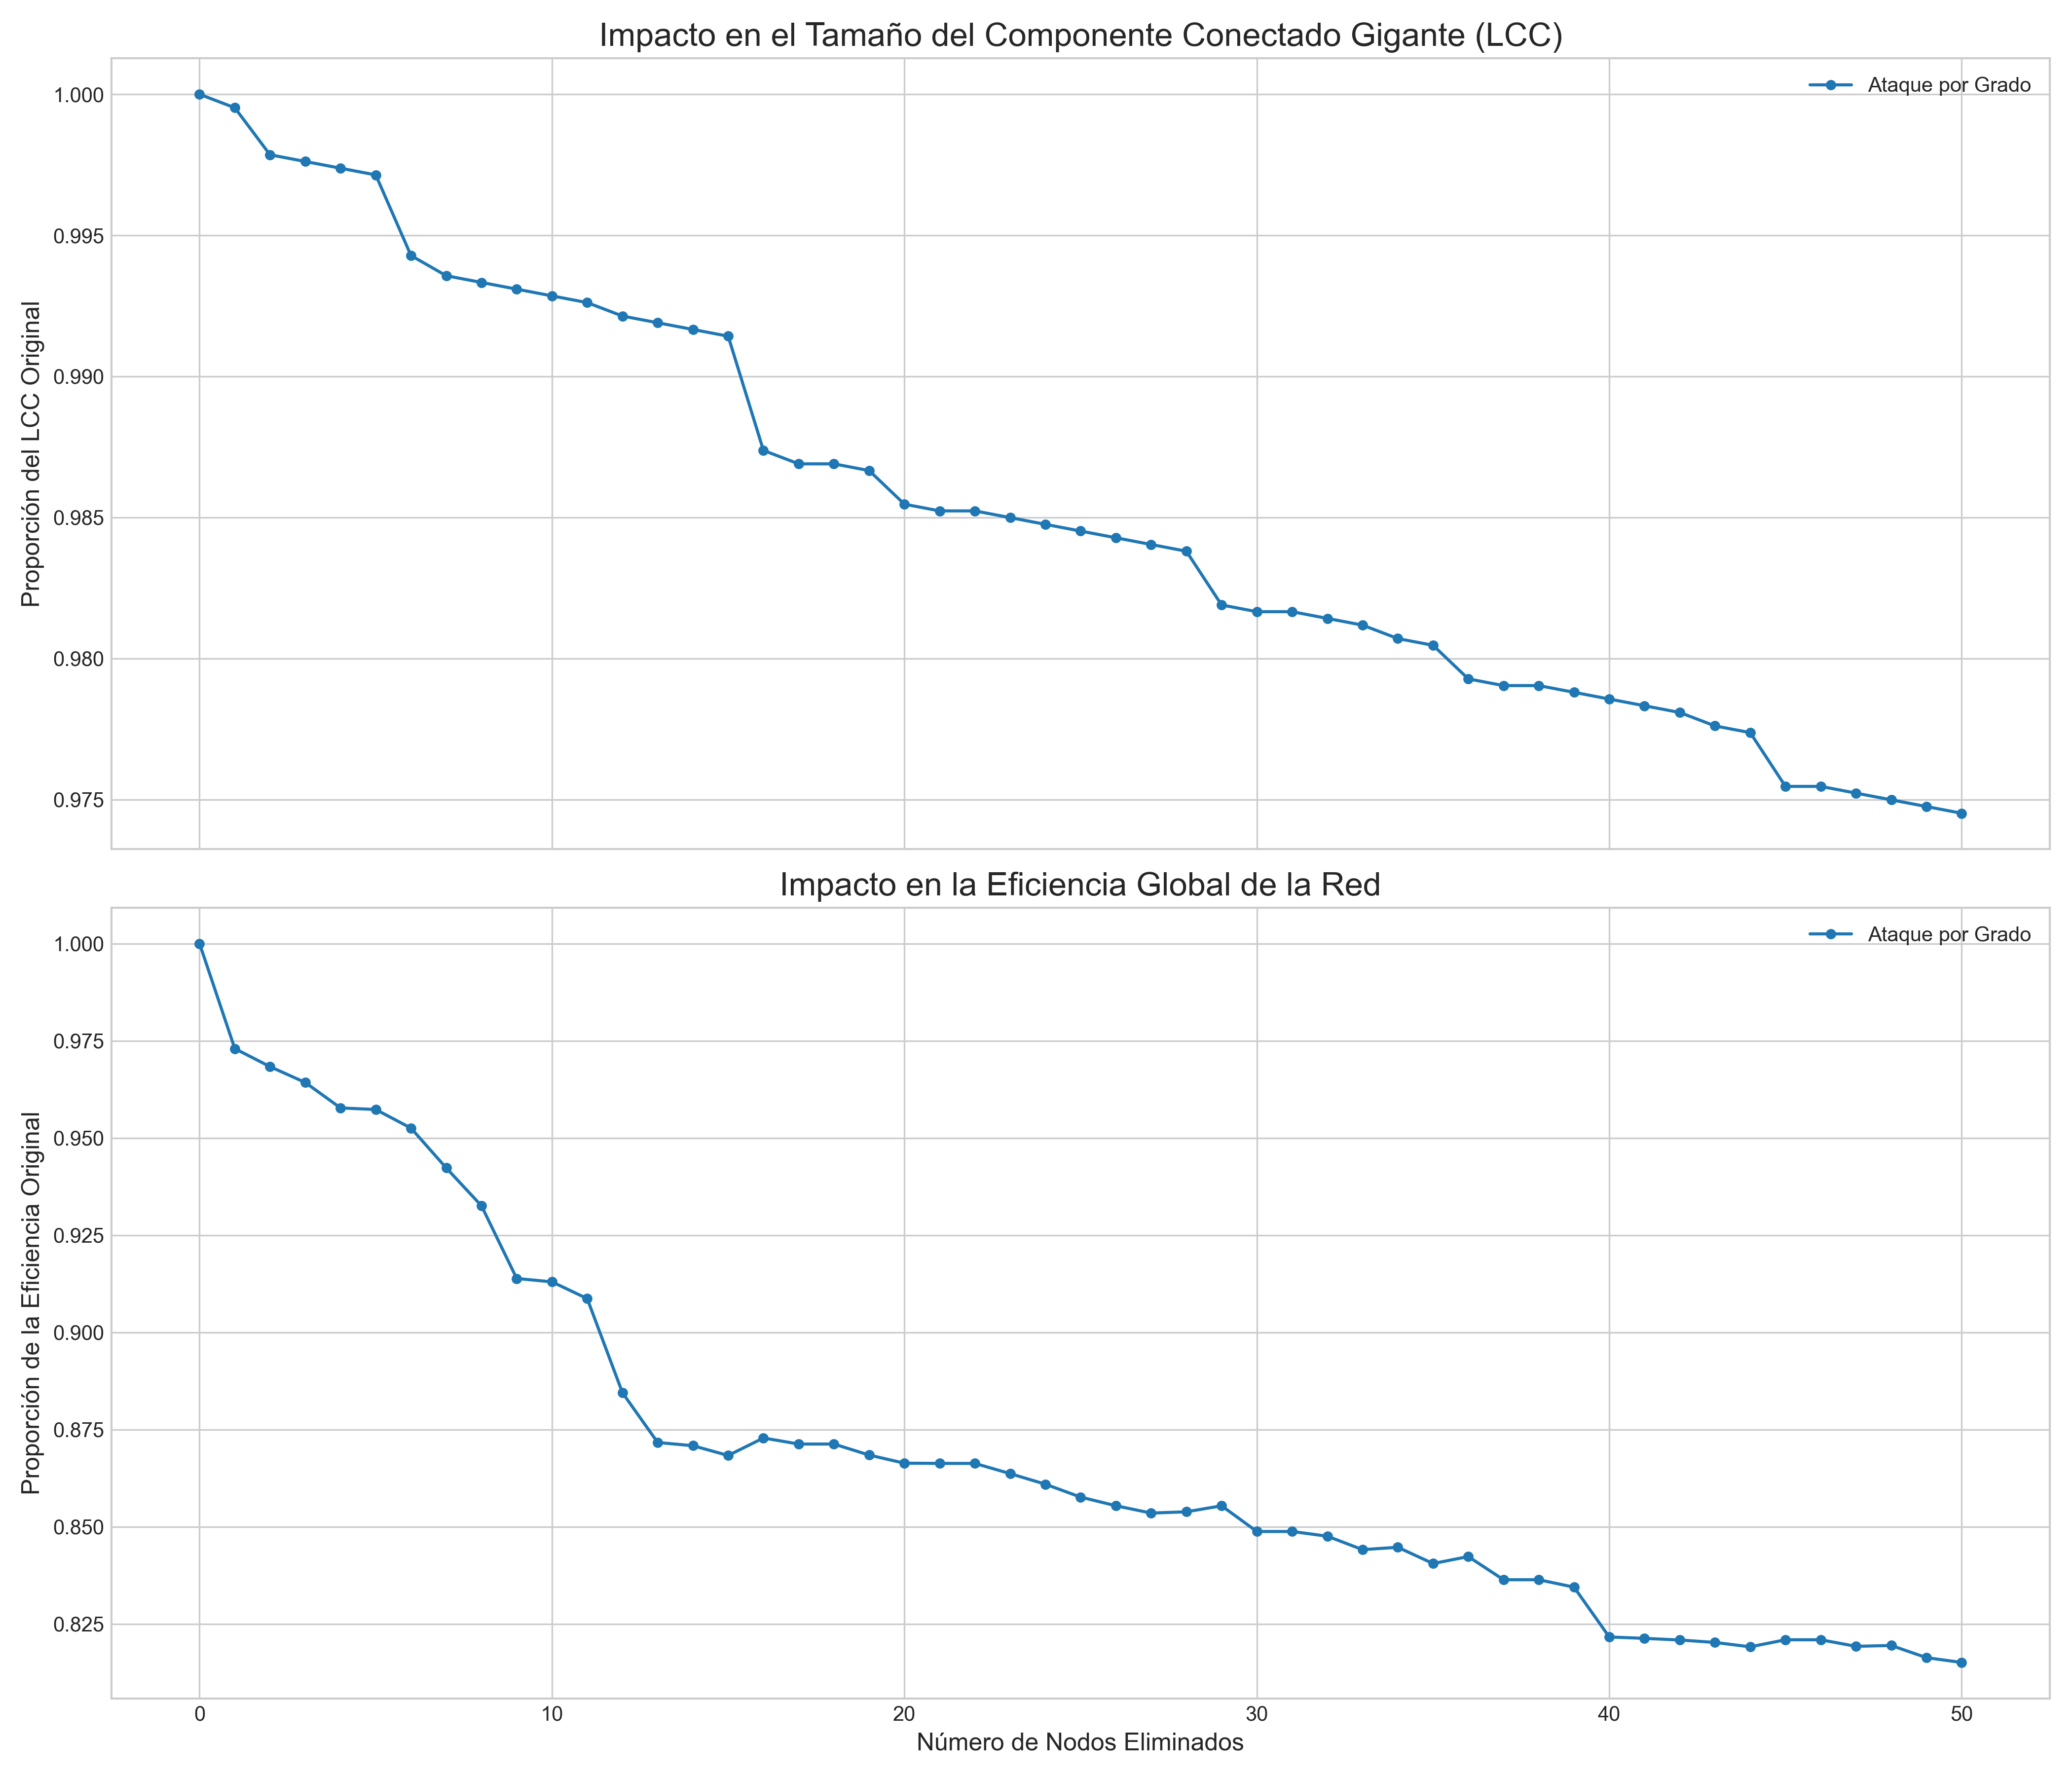
\includegraphics[width=\textwidth]{../../grafos/l_space/robustez/grafico_robustez_comparativo.png}
                \caption{Trayectorias del LCC relativo y de la eficiencia global del L-espacio durante la eliminación secuencial de 50 supernodos de mayor grado ponderado. Permite interpretar si el ataque dirigido compromete primero la cobertura de red o la calidad temporal de los recorridos.}
                \label{fig:robustez_l_space}
            \end{figure}

        \subsubsection{Impacto en la Conectividad (LCC)}
            En el escenario base de robustez (sin intervención), después de eliminar los 50 nodos de mayor grado ponderado, el LCC relativo conserva el \textbf{97.45\%} de su tamaño inicial. Esto indica que la red física mantiene la mayor parte de su cobertura estructural, aunque se generan pérdidas periféricas.

            Para mantener consistencia de lectura con la sección de intervenciones, conviene notar que allí se reporta el \(LCC\) post como porcentaje sobre nodos remanentes (\(98.51\%\) en la base), mientras que aquí se reporta la razón respecto al estado inicial (\(97.45\%\)).

        \subsubsection{Impacto en la Eficiencia Global}
            La eficiencia global cae al \textbf{81.50\%} de su valor original tras la eliminación de esos 50 nodos. Aunque la red sigue conectada, los caminos disponibles son menos directos y los tiempos de viaje promedio se alargan cerca de 18.50\%, lo que evidencia la dependencia operativa de los hubs de alto grado.

	\subsection{Conclusiones sobre el $L$-espacio}
	    El análisis permite concluir que la infraestructura del sistema en la Zona Metropolitana de Guadalajara tiene una estructura marcadamente arbórea, enfocada en conectar periferias con zonas centrales. Aunque el hipercentro concentra gran parte de la intermediación, también aparecen nodos de intersección relevantes fuera del centro, como estaciones del tren ligero y cruces comerciales estratégicos.

            En términos de robustez, la red conserva buena cobertura estructural bajo ataque dirigido, pero muestra una fragilidad temporal relevante: la eficiencia cae alrededor de \(18.50\%\) al remover 50 hubs. En otras palabras, la conectividad persiste, pero con recorridos más largos.

	    Ahora bien, este análisis no responde todas las preguntas sobre el servicio desde la perspectiva del usuario. Por ejemplo, la red anterior no permite estimar directamente cuántos transbordos son necesarios en los caminos evaluados. Para ello se requiere el grafo del $P$-espacio, que se analizó en el capítulo previo y se evalúa a continuación.

    \section{Análisis del P-espacio: La Red de Servicio}
        A continuación, se presentan los resultados del análisis aplicado al grafo P-espacio. Este modelo, donde los nodos se conectan si comparten una ruta, ofrece una perspectiva complementaria centrada en la experiencia de viaje del usuario sin transbordos.

        \subsection{Métricas globales del P-espacio}
            El grafo P-espacio es mucho más denso que el L-espacio:
            \begin{itemize}
                \item \textbf{Tamaño y densidad:} 4,203 nodos (supernodos) y 385,225 aristas (pares de supernodos que comparten al menos una ruta), con densidad \textbf{0.0436}.
                \item \textbf{Componentes:} 2 componentes; el principal reúne 4,198 supernodos.
                \item \textbf{Clustering:} Coeficiente de clustering global \textbf{0.4085}, lo que evidencia alta redundancia de rutas que comparten paradas.
                \item \textbf{Eficiencia y caminos:} Diámetro topológico \textbf{6} saltos y longitud promedio de camino \textbf{2.41} saltos (equivalentes a \textbf{hasta 5} y \textbf{1.41} transbordos, respectivamente, bajo la convención \textit{transbordos = saltos - 1}), con eficiencia global \textbf{0.4476} en el componente principal.
            \end{itemize}
	    Podemos ver que la densidad, casi dos órdenes de magnitud mayor que en el L-espacio, indica que la red de servicio ofrece muchas alternativas de conexión sin bajar de ruta en la adyacencia directa. El clustering elevado refleja cliques de paradas por rutas compartidas (redundancia operativa), mientras que un diámetro topológico de 6 y camino medio de 2.41 muestran que cualquier supernodo está a pocos pasos de otro, sugiriendo buena conectividad percibida por el usuario, aunque con riesgo de saturación en nodos altamente conectados. Algo interesante a notar es que un diámetro topológico de 6 implica que nuestra red es de \textit{mundo pequeño}, tal como lo predice la literatura para redes de este tipo.

        \subsection{Análisis de Centralidad en el P-espacio}
            Se calcularon y almacenaron las centralidades (grado, intermediación, cercanía y eigenvector). Los supernodos con mayor grado son aquellos que comparten numerosas rutas con otros supernodos, actuando como conectores de múltiples recorridos.

            Los cuatro indicadores coinciden en ubicar el máximo de centralidad en el hipercentro (Coords aprox. $20.668^{\circ}$ N, $-103.348^{\circ}$ O). Destacan:
            \begin{itemize}
                \item \textbf{Supernodo 264} (7 paradas). Top 1 en las cuatro métricas. Concentra al menos 30 rutas (ej. C05, C06, C111-V1/V3, C118) y funge como hub de transferencia natural en el centro.
                \item \textbf{Supernodo 262} (15 paradas) y \textbf{698} (5 paradas). También en el clúster central; comparten más de 25 rutas y aparecen en los primeros lugares de betweenness y cercanía.
                \item \textbf{Supernodos 1138 y 2117} (zona poniente; $\sim 20.646^{\circ}$ N, $-103.406^{\circ}$ O). Dominan eigenvector y cercanía en el sector occidental, con rutas como C104, C108, C123 y C124.
                \item Otros hubs relevantes: \textbf{2033}, \textbf{288} y \textbf{2073} (corredor central), y \textbf{151} en el oriente (C105, C106, C17).
            \end{itemize}
            En conjunto, la centralidad revela una red de servicio fuertemente articulada alrededor del centro histórico y varios corredores troncales, con abundante redundancia de rutas que permite mantener alta cercanía y conectividad incluso al remover nodos aislados.

            La pregunta para el servicio es: ¿qué supernodos concentran los transbordos más críticos y, por tanto, deben mantener prioridad operativa? La Figura~\ref{fig:centralidad_b_p_space} responde al escalar por grado y colorear por intermediación en el P-espacio, habilitando la priorización de puntos de transferencia.

            \begin{figure}[h!]
                \centering
                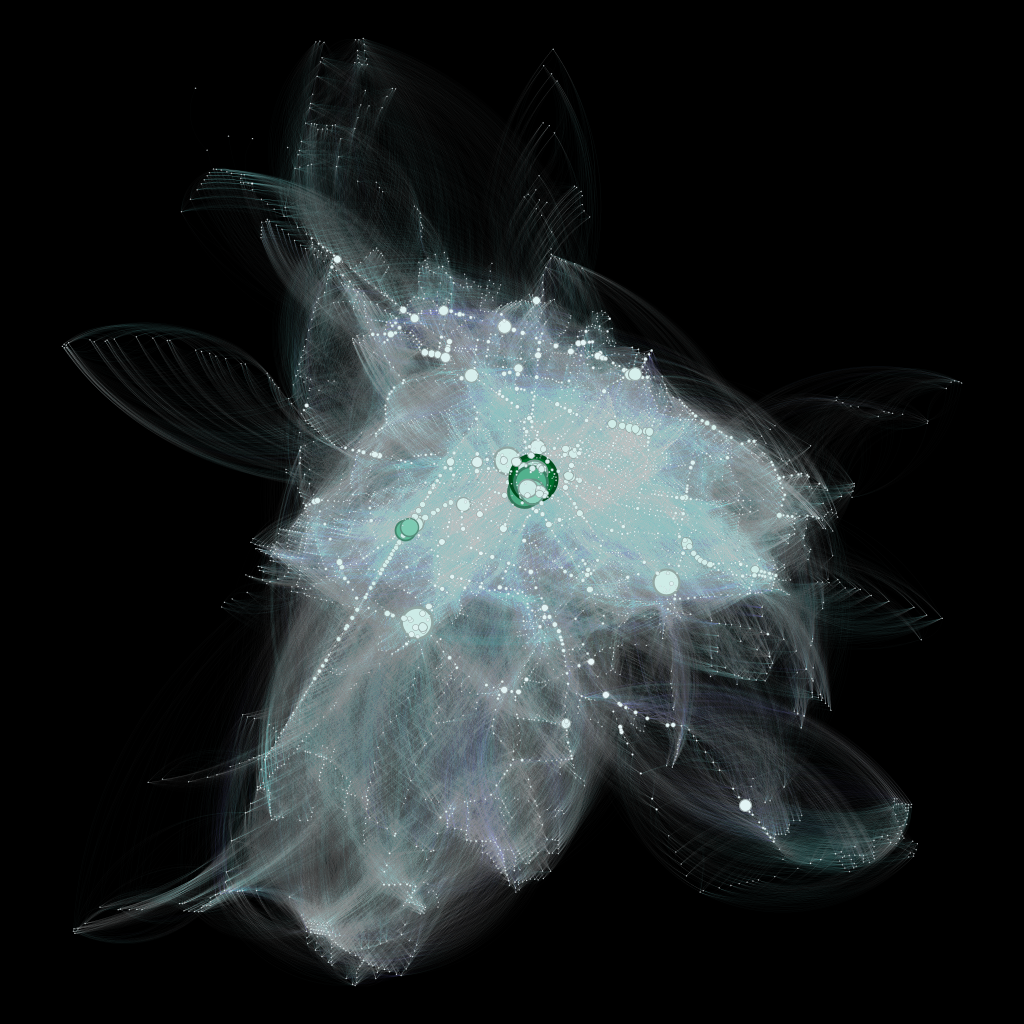
\includegraphics[width=\textwidth]{../../grafos/p_space/grafo_centralidades_betweness.png}
                \caption{P-espacio: tamaño del supernodo según grado y color verde según centralidad de intermediación. La combinación identifica supernodos de servicio que concentran rutas de transferencia y requieren prioridad operativa.}
                \label{fig:centralidad_b_p_space}
            \end{figure}

            La pregunta complementaria es: ¿desde qué supernodos se alcanza más rápido el resto del servicio y cuáles, además, se insertan en ejes influyentes? La Figura~\ref{fig:centralidad_c_p_space} responde al combinar cercanía y eigenvector, habilitando decidir dónde enfocar mejoras para acortar tiempos de viaje.

            \begin{figure}[h!]
                \centering
                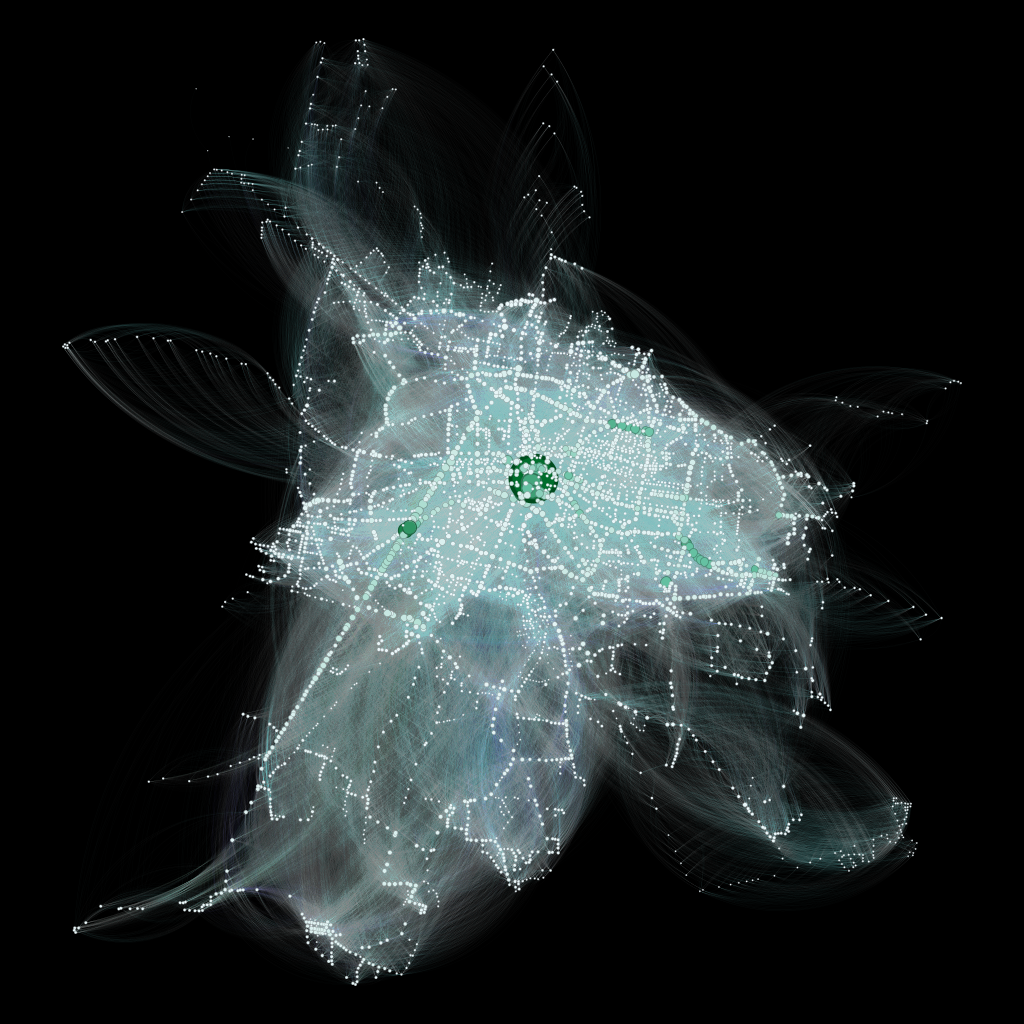
\includegraphics[width=\textwidth]{../../grafos/p_space/grafo_centralidades_closeness.png}
                \caption{P-espacio: color verde según centralidad de cercanía y tamaño del supernodo según centralidad de eigenvector. La lectura permite localizar ejes desde los cuales mejorar accesibilidad temporal con menor riesgo de afectar conectividad estructural.}
                \label{fig:centralidad_c_p_space}
            \end{figure}

        \subsection{Detección de Comunidades en el P-espacio}
            Se detectaron \textbf{11 comunidades} de supernodos mediante Louvain, agrupando paradas que comparten muchas rutas (modularidad $0.54$). Las cinco mayores concentran el 67\% de los supernodos del servicio:
            \begin{itemize}
                \item \textbf{Comunidad 5} (\textasciitilde\!18.2\%): centroide $(20.5748,-103.3608)$, domina el sur-poniente.
                \item \textbf{Comunidad 1} (\textasciitilde\!15.2\%): centroide $(20.6887,-103.2992)$, eje nororiente.
                \item \textbf{Comunidad 8} (\textasciitilde\!11.7\%): centroide $(20.7404,-103.3939)$, norponiente.
                \item \textbf{Comunidad 2} (\textasciitilde\!11.5\%): centroide $(20.6293,-103.2990)$, oriente-centro.
                \item \textbf{Comunidad 6} (\textasciitilde\!10.3\%): centroide $(20.6573,-103.2995)$, corredor central-oriente.
            \end{itemize}
            El resto incluye clusters poniente (Comunidad 4, 9) y núcleos menores (comunidades 0, 3, 7), mientras que sólo una comunidad es pequeña (\textless=5 nodos), reflejando alta conectividad transversal del servicio.

            La pregunta territorial en servicio es: ¿qué zonas comparten suficientes rutas para planear acciones coordinadas por comunidad? La Figura~\ref{fig:comunidades_p_space} responde al mostrar modularidad y aristas ponderadas por transbordos, habilitando decisiones de coordinación interzonal.

            \begin{figure}[h!]
                \centering
                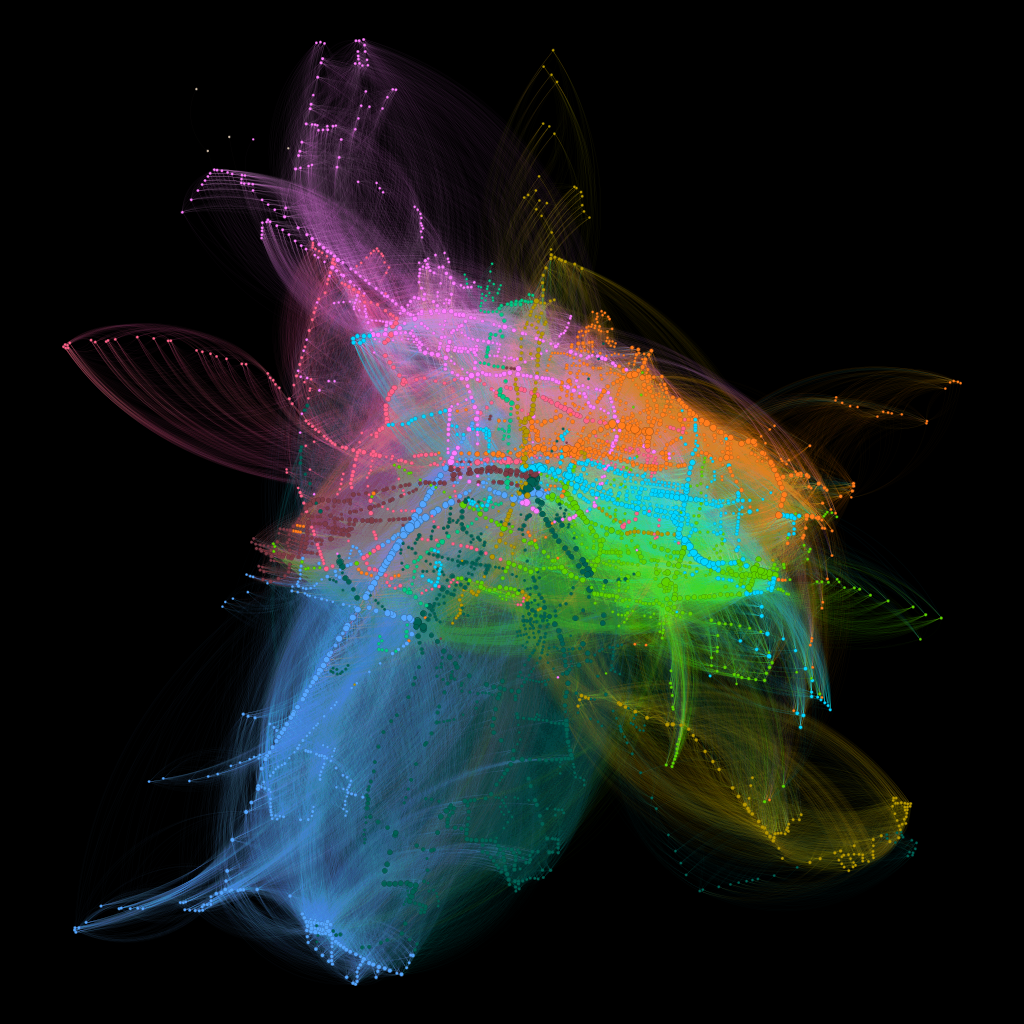
\includegraphics[width=\textwidth]{../../grafos/p_space/grafo.png}
                \caption{Comunidades del P-espacio detectadas con Louvain: color por comunidad y grosor de arista proporcional a la intensidad de transbordo entre supernodos. La figura apoya la priorización de estrategias coordinadas entre zonas funcionalmente conectadas.}
                \label{fig:comunidades_p_space}
            \end{figure}

        \subsection{Análisis de Robustez del P-espacio}
            Se aplicó el mismo esquema de ataque dirigido al P-espacio: eliminación secuencial de los \textbf{50 supernodos con mayor grado}. Tras cada eliminación se midieron el tamaño relativo del LCC y la eficiencia global no dirigida.

            La pregunta de resiliencia del servicio es: ¿la red pierde antes cobertura o eficiencia cuando fallan los supernodos de mayor grado? La Figura~\ref{fig:robustez_p_space} responde al comparar ambas trayectorias bajo el ataque dirigido, habilitando priorizar medidas de continuidad operativa.

            \begin{figure}[h!]
                \centering
                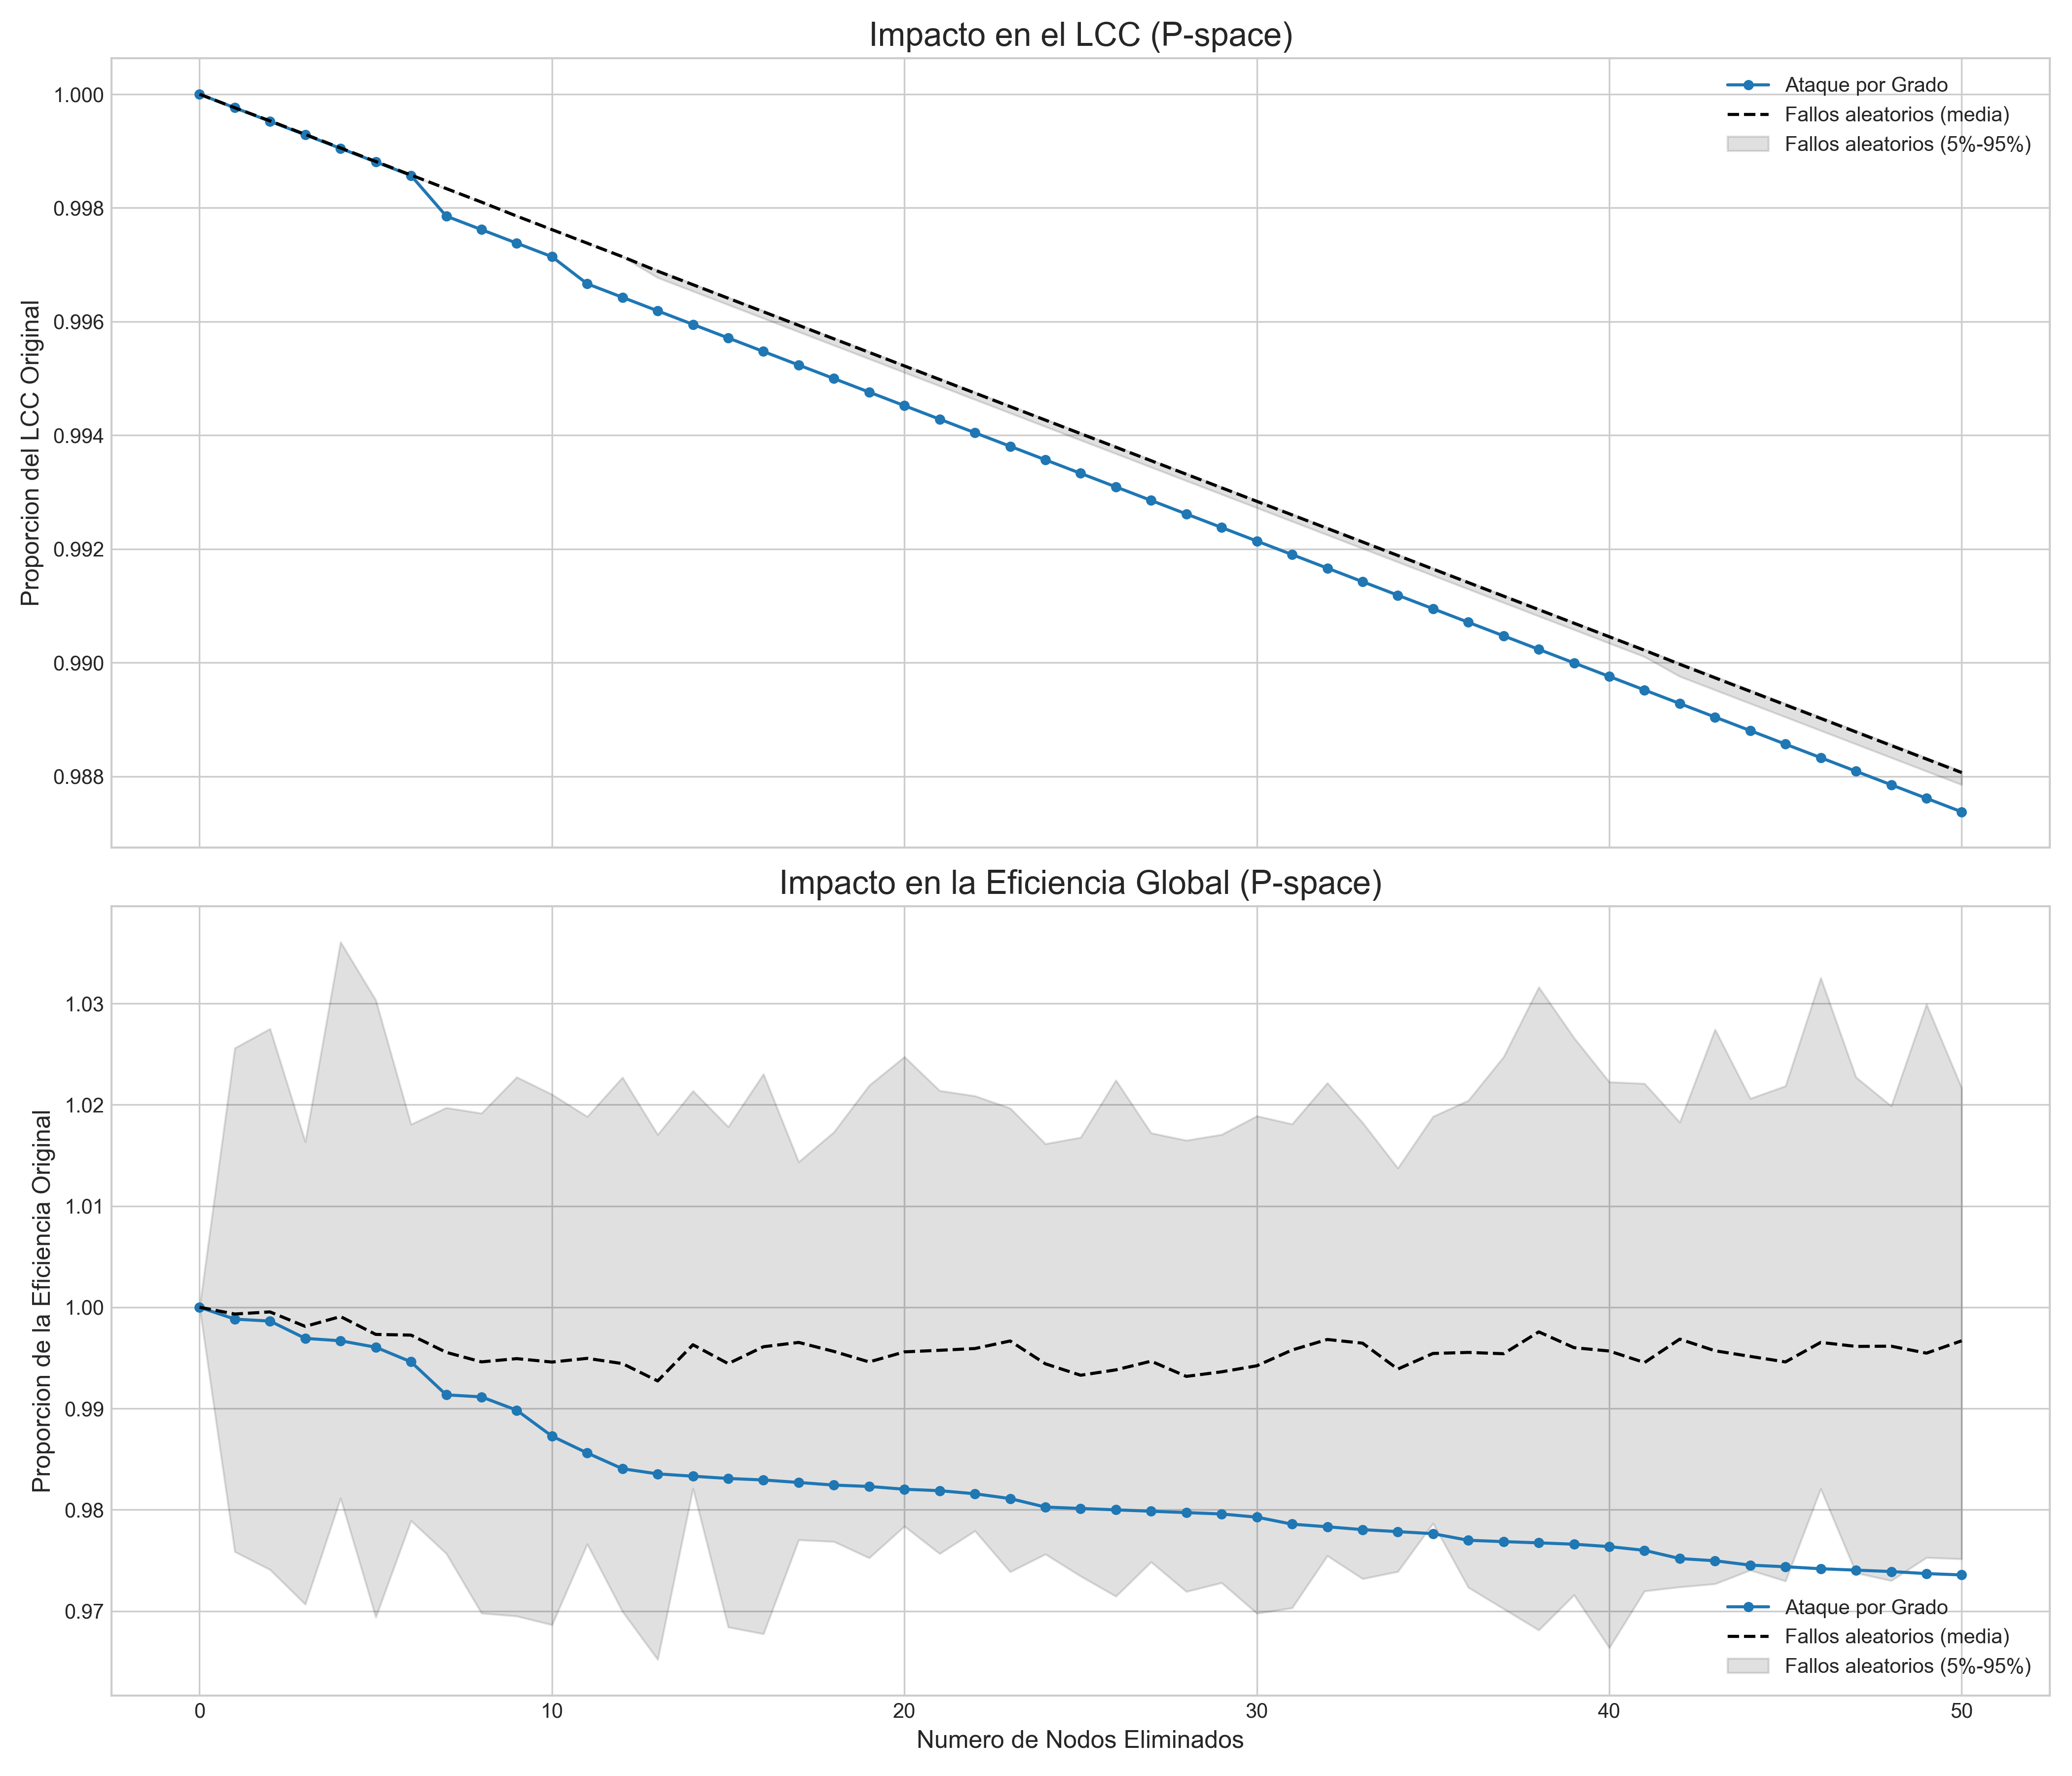
\includegraphics[width=\textwidth]{../../grafos/p_space/robustez/grafico_robustez_p_space_comparativo.png}
                \caption{Trayectorias del LCC relativo y de la eficiencia global del P-espacio durante la eliminación secuencial de 50 supernodos de mayor grado. Permite evaluar si la redundancia de servicio sostiene cobertura y/o rapidez ante fallas en nodos troncales.}
                \label{fig:robustez_p_space}
            \end{figure}

            Los resultados muestran que:
            \begin{itemize}
                \item El LCC se mantiene en \textbf{98.74\%} de su tamaño original tras eliminar los 50 supernodos más conectados, señal de alta redundancia en la red de servicio.
                \item La eficiencia global desciende a \textbf{97.36\%}, una caída moderada que sugiere que existen suficientes rutas alternativas para conservar recorridos relativamente cortos aun cuando fallan los hubs principales.
            \end{itemize}
            Comparativamente, el P-espacio es mucho más resiliente que el L-espacio: la pérdida de eficiencia es de apenas 2.64\% frente al 18.50\% observado en la infraestructura física. Esto se explica porque múltiples rutas comparten paradas y pueden sustituirse entre sí. Operativamente, el resultado sugiere que fallas en supernodos troncales se amortiguan si existen líneas paralelas o variantes, pero también que la redundancia descansa en el centro; un rediseño periférico podría mejorar la resistencia fuera del hipercentro.

        \subsection{Conclusiones sobre el $P$-espacio}
            Este modelo ofrece una perspectiva complementaria respecto al \(L\)-espacio. En términos generales, confirma que la red de servicio es densa, bien conectada y con rasgos de mundo pequeño. También muestra que, desde la experiencia del usuario, las zonas céntricas son todavía más determinantes que en la lectura puramente infraestructural.

            Asimismo, el \(P\)-espacio resulta resiliente ante cortes de servicio en supernodos de alto grado: la cobertura y la eficiencia se degradan de forma moderada, lo que sugiere alta redundancia de rutas y disponibilidad de alternativas para los usuarios.

    \section{Síntesis comparativa y validación del modelo}

        \subsection{Discusión Comparativa}
            El ataque dirigido por grado es significativamente más dañino en el L-espacio que en el P-espacio. Mientras que en la infraestructura física la eficiencia cae cerca de 18.50\% al perder 50 hubs, en la red de servicio la pérdida es de apenas 2.64\%. Esta comparación usa la misma métrica de eficiencia relativa al estado inicial en ambos grafos.

            Lo anterior confirma que la conectividad basada en compartir rutas es más resiliente por la existencia de múltiples combinaciones de servicio entre las paradas, aun si la infraestructura depende fuertemente de unos pocos nodos de alta interconexión.
	
        \subsection{Sensibilidad de Supuestos de Modelado}
            Para evaluar la estabilidad de los resultados, se ejecutó un análisis de sensibilidad con cuatro umbrales de consolidación espacial (\(75\), \(100\), \(125\) y \(150\) metros) y dos variantes para construir el \(P\)-espacio: clique por \texttt{route\_id} (modelo principal de la tesis) y clique por \texttt{trip\_id} (escenario conservador).

            En el \(L\)-espacio, al variar el umbral de consolidación cambia de forma importante el tamaño de la red, pero no su conectividad global: en todos los escenarios el componente gigante concentra más del \(99.8\%\) de los supernodos y no se observaron aristas con tiempo imputado.

            La pregunta metodológica es: ¿qué umbral de consolidación preserva la conectividad del L-espacio sin inducir fragmentación adicional? La Tabla~\ref{tab:sensibilidad_l_space} responde al comparar estructura y LCC por umbral, habilitando la decisión del rango de consolidación.

            \begin{table}[h!]
                \centering
                \caption{Sensibilidad del \(L\)-espacio ante el umbral de consolidación espacial (75--150 m): nodos, aristas, densidad, componentes y proporción del LCC. Sirve para seleccionar umbrales que preserven el componente gigante sin introducir fragmentación adicional.}
                \label{tab:sensibilidad_l_space}
                \begin{tabular}{lrrrrr}
                    \toprule
                    Umbral (m) & Nodos & Aristas & Densidad & Componentes & LCC (\%) \\
                    \midrule
                    75  & 5,084 & 9,550 & 0.000370 & 3 & 99.86 \\
                    100 & 4,203 & 8,591 & 0.000486 & 2 & 99.88 \\
                    125 & 3,360 & 7,442 & 0.000659 & 2 & 99.85 \\
                    150 & 2,676 & 6,280 & 0.000877 & 2 & 99.81 \\
                    \bottomrule
                \end{tabular}
            \end{table}

            En el \(P\)-espacio, la diferencia entre construir por \texttt{route\_id} y por \texttt{trip\_id} se mantiene en todos los umbrales: el enfoque por ruta produce más aristas, y entre \(8.73\%\) y \(20.86\%\) de ellas no aparecen en la variante por viaje.

            La pregunta de modelado es: ¿cuánto sesgo introduce construir el \(P\)-espacio por \texttt{route\_id} frente a \texttt{trip\_id} en cada umbral? La Tabla~\ref{tab:sensibilidad_p_space_route_trip} responde con el diferencial de aristas exclusivas del modelo por ruta, habilitando decidir el criterio de construcción más consistente con el objetivo analítico.

            \begin{table}[h!]
                \centering
                \caption{Comparación estructural del \(P\)-espacio construido por clique de \texttt{route\_id} frente a clique de \texttt{trip\_id}, con conteo de aristas exclusivas del modelo por ruta en cada umbral. Permite estimar el sesgo de sobreconectividad asociado al supuesto de agregación por ruta del modelo principal.}
                \label{tab:sensibilidad_p_space_route_trip}
                \begin{tabular}{lrrrr}
                    \toprule
                    Umbral (m) & Aristas route\_id & Aristas trip\_id & Exclusivas por ruta & Exclusivas por ruta (\%) \\
                    \midrule
                    75  & 517,964 & 409,923 & 108,041 & 20.86 \\
                    100 & 385,225 & 325,855 & 59,370  & 15.41 \\
                    125 & 269,642 & 239,093 & 30,549  & 11.33 \\
                    150 & 182,926 & 166,955 & 15,971  & 8.73 \\
                    \bottomrule
                \end{tabular}
            \end{table}

            En conjunto, el análisis muestra dos cosas: (i) las conclusiones cualitativas principales (presencia de un componente gigante y alta conectividad de servicio) son robustas al rango de umbrales evaluado; (ii) las magnitudes de densidad y cantidad de aristas sí son sensibles al supuesto de consolidación y al criterio de construcción por ruta o por viaje en \(P\)-espacio, por lo que en adelante se reportan como rangos y no como un único valor puntual.

        \subsection{Escenarios de Intervención Topológica}
            Para convertir el diagnóstico estructural en propuestas comparables, se evaluaron tres intervenciones sobre el \(L\)-espacio y se contrastaron con un escenario base sin cambios:
            \begin{itemize}
                \item \textbf{Protección de hubs:} se inmunizan los 10 supernodos de mayor grado ponderado y se aplica el mismo ataque dirigido de 50 nodos sobre el resto.
                \item \textbf{Refuerzo periférico:} se agregan 120 aristas dirigidas (60 pares bidireccionales) entre nodos de baja cercanía para crear atajos periféricos.
                \item \textbf{Recableado con bypass:} se agregan 200 aristas de bypass alrededor de hubs para introducir rutas alternativas entre vecinos de nodos troncales.
            \end{itemize}
            En los cuatro escenarios se aplicó el mismo ataque dirigido: eliminación secuencial de los 50 supernodos con mayor grado ponderado. Después del ataque se midieron tres indicadores: \(LCC\) post sobre nodos remanentes, eficiencia global dirigida (ponderada por \texttt{travel\_time\_minutes}) y diámetro topológico del componente gigante.

            La pregunta de decisión es directa: ¿qué intervención conserva mejor la conectividad y, al mismo tiempo, evita que los recorridos se vuelvan mucho más largos tras el ataque? La Tabla~\ref{tab:intervenciones_topologicas_l_space} responde al comparar las métricas post-ataque para cada escenario.

            \begin{table}[h!]
                \centering
                \small
                \caption{Escenarios de intervención topológica en \(L\)-espacio después de un ataque dirigido de 50 supernodos: aristas agregadas, LCC post-ataque, retención de eficiencia y diámetro. La tabla permite comparar el balance entre resiliencia estructural y desempeño temporal de cada estrategia.}
                \label{tab:intervenciones_topologicas_l_space}
                \resizebox{\textwidth}{!}{%
                \begin{tabular}{lrrrrr}
                    \toprule
                    Escenario & Aristas nuevas & LCC post (\%) & Retención de eficiencia (\%) & Diámetro post & \(\Delta\)LCC vs base (pp) \\
                    \midrule
                    Base (sin intervención) & 0   & 98.51 & 82.50 & 84 & 0.00 \\
                    Protección de hubs      & 0   & 99.30 & 85.58 & 97 & +0.79 \\
                    Refuerzo periférico     & 120 & 98.51 & 88.52 & 53 & +0.00 \\
                    Recableado con bypass   & 200 & 98.82 & 79.68 & 84 & +0.31 \\
                    \bottomrule
                \end{tabular}%
                }
            \end{table}

            La comparación muestra que cada intervención favorece un aspecto distinto de la resiliencia:
            \begin{itemize}
                \item \textbf{Protección de hubs} es la mejor opción para preservar conectividad: eleva el \(LCC\) post-ataque de \(98.51\%\) a \(99.30\%\). Sin embargo, esa mejora viene acompañada de un diámetro mayor (de 84 a 97), es decir, la red residual queda más unida pero más alargada.
                \item \textbf{Refuerzo periférico} ofrece el mejor balance operativo: mantiene el \(LCC\) al nivel del escenario base, pero logra la mayor retención de eficiencia (\(88.52\%\) frente a \(82.50\%\)) y reduce el diámetro de 84 a 53. En términos prácticos, conserva recorridos más cortos después del ataque.
                \item \textbf{Recableado con bypass} sólo aporta una mejora marginal en conectividad (\(+0.31\) pp en \(LCC\)), pero reduce la eficiencia relativa a \(79.68\%\), por debajo del escenario base. En su forma actual, no justifica su costo estructural y requeriría una regla de diseño más afinada.
            \end{itemize}
            En conjunto, la evidencia sugiere priorizar \textbf{refuerzo periférico} cuando el objetivo principal es sostener tiempos de recorrido razonables bajo falla, y \textbf{protección de hubs} cuando se busca maximizar la conectividad residual. Ambas estrategias resultan más defendibles que el recableado con bypass y, además, reducen la dependencia exclusiva del hipercentro.

        \subsection{Bandas de Incertidumbre de Resultados}
            Para evitar depender de un único valor puntual, se consolidaron los resultados de los puntos 3 y 4 en términos de bandas mínimo--máximo. Esto permite separar dos efectos: (i) la variación por supuestos de modelado (umbral de consolidación y criterio \texttt{route\_id}/\texttt{trip\_id}); y (ii) la variación por decisiones de intervención bajo un mismo ataque dirigido.

            La pregunta de incertidumbre es: ¿qué métricas permanecen estables y cuáles varían materialmente según supuestos e intervenciones? La Tabla~\ref{tab:rangos_consolidados_p3_p4} responde al sintetizar mínimos, máximos y amplitudes, habilitando decidir qué indicadores requieren monitoreo prioritario.

            \begin{table}[h!]
                \centering
                \small
                \caption{Rangos mínimo--máximo de métricas clave en los puntos 3 (modelado) y 4 (intervenciones), con amplitud por indicador. La síntesis permite identificar qué resultados son robustos y cuáles dependen del supuesto de modelado o de la intervención.}
                \label{tab:rangos_consolidados_p3_p4}
                \begin{tabular}{llrrr}
                    \toprule
                    Bloque & Métrica & Mín & Máx & Amplitud \\
                    \midrule
                    P3 (modelado) & L-space nodos & 2,676 & 5,084 & 2,408 \\
                    P3 (modelado) & L-space aristas & 6,280 & 9,550 & 3,270 \\
                    P3 (modelado) & LCC L-space (\%) & 99.81 & 99.88 & 0.07 \\
                    P3 (modelado) & Exclusivas por ruta en P-space (\%) & 8.73 & 20.86 & 12.13 \\
                    P4 (intervenciones) & LCC post-ataque (\%) & 98.51 & 99.30 & 0.79 \\
                    P4 (intervenciones) & Retención de eficiencia (\%) & 79.68 & 88.52 & 8.85 \\
                    P4 (intervenciones) & Diámetro post-ataque (saltos) & 53 & 97 & 44 \\
                    \bottomrule
                \end{tabular}
            \end{table}

            Los rangos muestran que la \textbf{conectividad global} de la red física es estable frente a los supuestos de consolidación (\(LCC\) de \(99.81\%\) a \(99.88\%\)); en cambio, la magnitud de \textbf{sobrerepresentación potencial} en \(P\)-espacio (aristas exclusivas del modelo por ruta) cambia de manera importante (\(8.73\%\) a \(20.86\%\)). Bajo ataque dirigido, las intervenciones producen diferencias operativas relevantes: la retención de eficiencia varía entre \(79.68\%\) y \(88.52\%\), y el diámetro post-ataque entre 53 y 97 saltos.

            La pregunta final es: ¿la amplitud de las bandas altera o confirma la priorización entre escenarios de intervención? La Figura~\ref{fig:rangos_intervenciones_punto4} responde al comparar visualmente los rangos por escenario, habilitando sustentar decisiones aun bajo incertidumbre estructural.

            \begin{figure}[h!]
                \centering
                \IfFileExists{../../out/incertidumbre/punto5_rangos/rangos_intervenciones_punto4.png}{
                    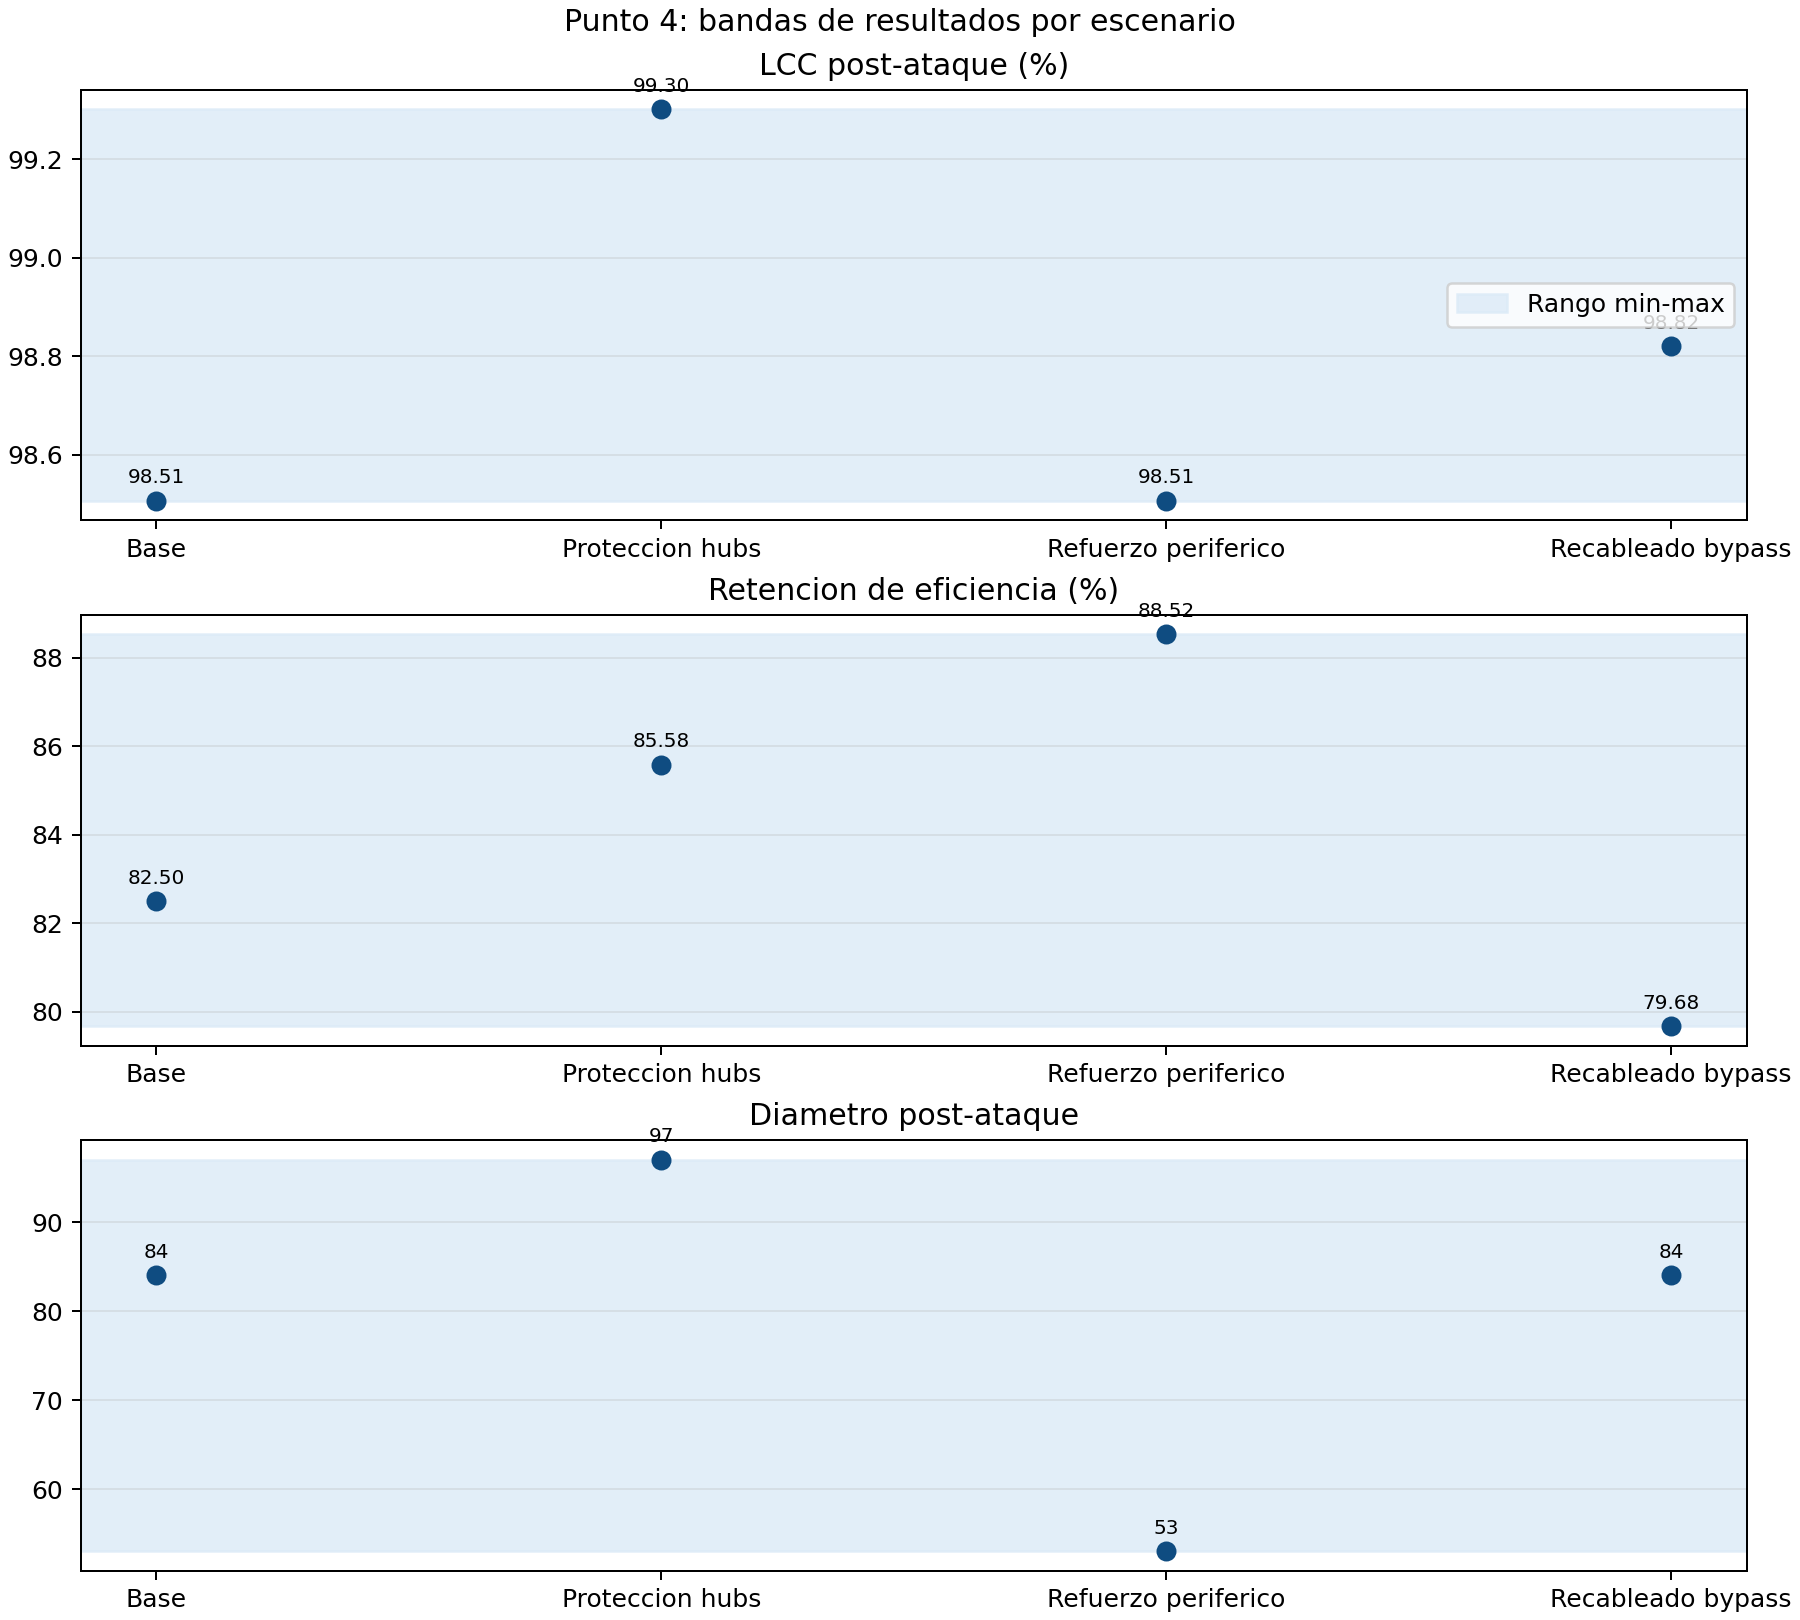
\includegraphics[width=\textwidth]{../../out/incertidumbre/punto5_rangos/rangos_intervenciones_punto4.png}
                }{
                    \fbox{\parbox{0.92\textwidth}{Generar figura con: \texttt{python "Código/analisis\_comparativo/rangos/analisis\_rangos\_resultados.py"}}}
                }
                \caption{Bandas mínimo--máximo por escenario de intervención topológica en \(L\)-espacio (punto 4). La figura permite evaluar si la incertidumbre entre escenarios altera la priorización de decisiones de intervención.}
                \label{fig:rangos_intervenciones_punto4}
            \end{figure}

            En síntesis, la tesis mantiene sus conclusiones cualitativas centrales, pero las magnitudes clave se reportan en adelante como rangos para reflejar explícitamente la incertidumbre estructural del modelado.

    \section{Parámetros, Software y Reproducibilidad}

        Para garantizar la transparencia y la posibilidad de replicar los hallazgos de este capítulo, a continuación se detallan el software, los parámetros y los datos utilizados.

        \subsection{Convenciones de Notación y Redondeo}
            Para mantener consistencia editorial en toda la tesis, se emplean las siguientes convenciones:
            \begin{itemize}
                \item \textbf{Supernodo:} nodo agregado por consolidación espacial (DBSCAN).
                \item \textbf{Arista y arco:} en los capítulos aplicados se usa \emph{arista} como término general; \emph{arco} se reserva para el formalismo dirigido cuando la orientación es explícita.
                \item \textbf{Salto vs. transbordo:} un \emph{salto} es una arista recorrida en el grafo; un \emph{transbordo} es un cambio de ruta. En \(P\)-espacio se aproxima por \(\text{transbordos}=\text{saltos}-1\).
                \item \textbf{Redondeo:} conteos y diámetros se reportan como enteros; porcentajes con dos decimales; métricas continuas en \([0,1]\) con cuatro decimales (o seis decimales cuando el valor es muy pequeño, como densidad en \(L\)-espacio).
            \end{itemize}

        \subsection{Software y Hardware}

            El análisis estructural de la red se llevó a cabo utilizando el lenguaje de programación \textbf{Python 3}. Las principales librerías empleadas fueron:
            \begin{itemize}
                \item \textbf{NetworkX:} Para la creación, manipulación y análisis del grafo, incluyendo el cálculo de todas las métricas de centralidad, componentes conectados y eficiencia.
                \item \textbf{Pandas:} Para la manipulación de los datos y la gestión de los resultados de las simulaciones.
                \item \textbf{Matplotlib} y \textbf{Seaborn:} Para la generación de las visualizaciones y gráficos.
                \item \textbf{NumPy:} Para operaciones numéricas y el manejo de arreglos.
                \item \textbf{Multiprocessing:} Para la paralelización del cálculo de la eficiencia global, optimizando significativamente el tiempo de ejecución.
            \end{itemize}
            Los cálculos se realizaron en un equipo de escritorio estándar. El uso de la paralelización, que distribuye la carga de trabajo entre múltiples núcleos de CPU, fue crucial para completar el análisis de robustez en un tiempo razonable.

        \subsection{Parámetros del Análisis}

            \begin{itemize}
                \item \textbf{Centralidades:} Para los cálculos de centralidad se utilizaron los pesos de las aristas correspondientes:
                \begin{itemize}
                    \item \textbf{Intermediación y Cercanía:} Se utilizó como peso el tiempo de viaje en minutos para encontrar los caminos más rápidos.
                    \item \textbf{Grado Ponderado:} Se calculó como la suma del grado de entrada ponderado y del grado de salida ponderado, que representan el número de rutas que pasan por un nodo.
                \end{itemize}
                \item \textbf{Detección de Comunidades:} Se empleó el método de Louvain, optimizando la modularidad sobre una versión no dirigida del grafo ponderado por el número de rutas.
                \item \textbf{Análisis de Robustez:}
                \begin{itemize}
                    \item Se eliminaron secuencialmente los \textbf{50 nodos de mayor grado} en cada grafo (L-espacio y P-espacio).
                    \item El cálculo de la eficiencia global se realizó de forma exacta y paralelizada (L-espacio) o con la función nativa de NetworkX (P-espacio).
                \end{itemize}
            \end{itemize}

        \subsection{Reproducibilidad}

            El código fuente completo desarrollado para este análisis, incluyendo los scripts para la construcción del grafo, el cálculo de métricas y las simulaciones de robustez, se encuentra disponible en el repositorio digital citado en las referencias.
